%%%%%%%%%%%%%%%%%%%%%%%%%%%%%%%%%%%%%%%%%%%%%%%%%%%%%%%%%%%%%%%%%%%%%%%%%%%%%
\section{GPGPU Introduction}

GPGPU (\textit{General Purpose computation on Graphics Processor Unit}), also known as \textit{GPU Computing}, is the utilization of the graphic adapter of a personal computer to perform generic and non-graphic related computation usually handled by the CPU.\\
Once designed and optimized specifically to perform only graphic calculations, modern GPUs are evolving into \emph{high-performances many-core} processors that can be virtually used to perform any task, and developers who port their applications to GPUs are able to achieve speedups of orders of magnitude vs. optimized CPU implementations.\cite{GPGPUORG:About}\\
The reason why GPUs are so fast has to be searched [.... ... ] GPUs were born to deal with [extensive performace request by videogame]
Ottimizzate per fare poche e semplici operazioni su vertici e matrici, ma in PARALLELO -> parallelismo intriseco.
GPUs have been built to exploit application parallelism, and a single graphic adapter can host hundreds, if not thousands, of cores; this translates in TeraFlops of operations per second vs. the few GigaFlops a CPU can handle alone.//
 (incremento pi� alto di legge di moore?)

\begin{figurehere}
 \centering
 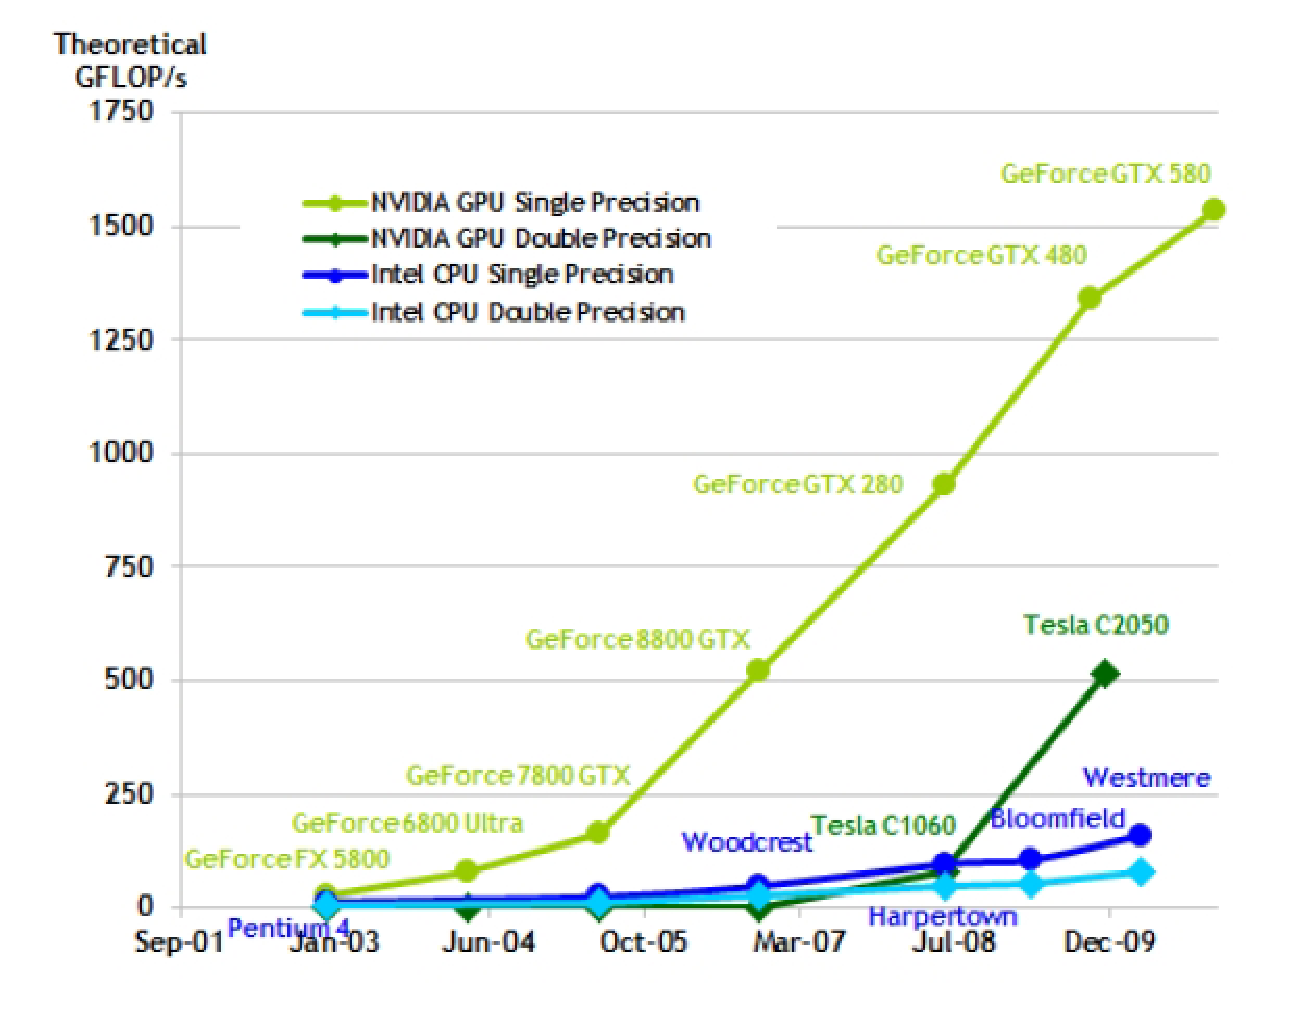
\includegraphics[width=8cm, height=4cm]{./eps/GPU_CPU_chart.eps}
 \caption{CPU vs GPU growth rate.}
 \label{fig:cpuvsgpu}
\end{figurehere}


-esempi applicativi
Due to its parallel nature, GPU computing can be very effective for applications involving huge amount of data, especially if the data can be structured in structures like vectors and arrays.
Parallel GPU computation can be applied in various applications and research-field, from computer vision, to mathematical simulations, to bio-informatics, often allowing to achieve in few months results that would have required years with a standard CPU-only approach (with speedups of even 250x,350x).

METTERE GRAFICO DEL PAPER??

As seen in TAB, GPU can offload the CPU from most of its work, but this doesn't mean that CPU performance is no longer critical. Many applications don't (and can't) map all their code to the GPU, and in certain cases the CPU can run some part of the code more effectively than the GPU.
Furthermore, not all the code can be mapped easily and clearly on the GPU, as programming in this say can be way more difficult than programming in a standard way, it is not possible to simply "`port"' the code from the CPU to the GPU.
-problemi: difficolt�

%-----------------------------------------------------------------------------
\subsection{Basic Principles}
% Please avoid separations in titles
% and separate text manually

In this section we'll analyze some of the basic principles behind GPGPU programming. Some of these concepts are directly related to and help to understand why GPU computing is so fast, for instance, GPUs can handle bidimensional matrices natively, while CPUs are limited to single dimension array.
A GPU is basically a \textit{stream processor}: a \textbf{kernel} is executed over a stream of data in a monolitic fashion.
Thanks to the GPU architecture, the data can be elaborated in parallel, and more than one kernel can be running at the same time. (VERIFICARE?)

\subsubsection{Textures = Arrays}
Due to the linear structure of memory, traditional CPUs cannot \emph{physically} create multi-dimensional array, and accessing rows and columns of a simple matrix is obtained by offsetting coordinates in a large one-dimensional array, each "`jump"' in memory translates in performance loss.
GPUs are architectured to work natively with textures, that can be seen as two-dimensional array. One drawback is that the amount of memory on graphics adapters is limited, compared to the system RAM available to the CPU, and for this reason most of the GPUs can work only with textures of a limited size. The usual maximum size of a texture is usually 2048*2048, or 4096*4096, but modern can reach sizes of 8192*8192.
The maximum texture size available for a certain graphic adapter can usually be retrieved by simple queries made available by the API you are using.

\begin{CLCode}
In OpenCL, you can obtain the maximum supported texture size with the \textsl{clGetDeviceInfo()} function, passing the
\textsl{CL\_DEVICE\_IMAGE2D\_MAX\_WIDTH} and \textsl{CL\_DEVICE\_IMAGE2D\_MAX\_HEIGHT} parameters.
\end{CLCode}

We will discuss how textures are created and accessed more in deep in Section \ref{}, when we will introduce the OpenCL API.

\begin{itemize}
	\item Array \= Texture
	\item Kernels
	\item Feedback
	\item ....
\end{itemize}


%This is a citation \cite{Norman09Learn} and here is another citation
%\cite{Peyton93Howto}.  Lorem ipsum dolor sit amet, consectetur adipiscing elit.


%And this is the reference to a single column figure (see {\bf Figure
%\ref{fig:myfigure1}}).  Lorem ipsum dolor sit amet, consectetur adipiscing elit.

\begin{figurehere}
 \centering
 \includegraphics[width=8cm, height=4cm]{./eps/placeholder.eps}
 \caption{Some single-column figure caption.}
 \label{fig:myfigure1}
\end{figurehere}


%-----------------------------------------------------------------------------
\subsection{GPGPU Programming Languages}


\begin{figure*}[t]
  \centering
 \includegraphics[width=16cm, height=4cm]{./eps/placeholder.eps}
 \caption{Some wide-figure caption.}
 \label{fig:myfigure2}
\end{figure*}

And this is the reference to a single column figure (see {\bf Figure
\ref{fig:myfigure2}}). Lorem ipsum dolor sit amet, consectetur adipiscing elit.

%%%%%%%%%%%%%%%%%%%%%%%%%%%%%%%%%%%%%%%%%%%%%%%%%%%%%%%%%%%%%%%%%%%%%%%%%%%%%